\documentclass[conference]{IEEEtran}
\IEEEoverridecommandlockouts
% The preceding line is only needed to identify funding in the first footnote. If that is unneeded, please comment it out.
\usepackage{cite}
\usepackage{comment}
\usepackage{amsmath,amssymb,amsfonts}
\usepackage{algorithmic}
\usepackage{hyperref}
\usepackage{graphicx}
\usepackage{textcomp}
\usepackage{xcolor}
\usepackage{subcaption}
\usepackage{multirow}
\usepackage{booktabs}
\usepackage{caption}
\usepackage{tabularx}
\usepackage{ragged2e}
\usepackage{makecell}
\usepackage{array}
\usepackage{xcolor}
\usepackage{adjustbox}

\def\BibTeX{{\rm B\kern-.05em{\sc i\kern-.025em b}\kern-.08em
    T\kern-.1667em\lower.7ex\hbox{E}\kern-.125emX}}
\begin{document}

\title{\textcolor{blue}{[WORKSHOP]}Towards Greener Networks: RApp-Based Cell Control over O-RAN Deployments}

\author{\IEEEauthorblockN{1\textsuperscript{st} Given Name Surname}
\IEEEauthorblockA{\textit{dept. name of organization (of Aff.)} \\
\textit{name of organization (of Aff.)}\\
City, Country \\
email address or ORCID}
}

\maketitle

\begin{abstract}
Write at the end. Highlight the problem statement, contribution, novelty, and one/two imp results.
\end{abstract}

\begin{IEEEkeywords}
Keywords.
\end{IEEEkeywords}

\section{Good Lines}
- While a mobile network consists of multiple parts, the radio access network (RAN) is responsible for most of the energy consumption in a mobile network. ==> 
Green Future Networks – Sustainability Challenges and Initiatives in Mobile Networks by NGMN Alliance,
December 2021
\href{https://www.ngmn.org/wp-content/uploads/210719_NGMN_GFN_Sustainability-Challenges-andInitiatives_v1.0.pdf} \\
- A radio access network comprises of several cell sites with site infrastructure equipment and base station equipment. \\
- O-RAN can contribute to this effort immensely. Its disaggregated and virtualized architecture adds complexity; however, energy is the next major challenge O-RAN must overcome. \\
- Rimedo Labs recently released Energy Saving rApp (ES-rApp) for Non-RT RIC focusing on Massive MIMO use cases. \\ 
\\
- The RF carrier shutdown feature (typically hosted by the SMO and non-RT RIC in O-RAN architecture)
periodically checks the service load of multiple carriers and if the service load is below a specified threshold, the capacity-layers are shut off (see Figure 12). The UEs served by those carriers can camp on or access the services from the carrier providing basic coverage. When the load of the carrier providing basic coverage is higher than a specified threshold, the base station turns on the carriers that have been shut down for service provisioning. \\
- RF carriers can be shut down by non-RT RIC rAPPs more intelligently using information from telemetry data from E2 interface with O-RAN.\\
- Switching off under-loaded cells during network operation without affecting the user experience (call drops, QoS degradation, etc.) is one way to achieve RAN energy efficiency. \\
- A typical energy savings scenario is realized when capacity booster cells are deployed under the umbrella of cells providing basic coverage and the capacity booster cells are switched off to enter dormant mode when its capacity is no longer needed and reactivated on a need basis. \\
- When the booster gNB with CU/DU split decides to switch off cell(s) to the dormant state, the decision is typically made by the gNB-DU based on cell load information or by the OAM entity (non-RT RIC in O-RAN architecture). Before the cell in the gNB-DU enters into the dormant mode, the gNB-DU will send the gNB-DU configuration update message to the gNB-CU to indicate that the gNB-DU will switch off the cell subsequently sometime later. \\ 
- \textcolor{blue}{During the switch-off period, the gNB-CU offloads the UE to a neighboring cell and simultaneously will not admit any incoming UE to this cell being switched-off. Is this load balancing performed?}\\
- https://networkbuilders.intel.com/solutionslibrary/a-holistic-study-of-power-consumption-and-energy-savings-strategies-for-open-vran-systems \\ 
\\
- RF channel switch off/on \\
- \textcolor{blue}{However, the switch off/on decisions are need a lot of KPIs reporting and efficient actions so that guarantee the overall user experience. Also, there are conflicting targets between system performance and energy savings.} \\
\\
- \textcolor{blue}{Offline learning is normally preferred (including reinforcement learning which is usually performed online) due to the nature of the network environment, which is prone to misconfiguration and errors leading to outages. The proposed approach is for the model to first be trained with offline data and that the trained model then be deployed in the network for inference.} 
- \textcolor{blue}{ES-rApp aims at minimizing the overall energy consumption by switching off cells that are not loaded too much, and turning on the cells if the traffic load goes high.}\\
- \textcolor{blue}{If the shift of all the users from a given cell is possible (i.e., if the performance requirements of already served users can be guaranteed), it generates the appropriate policy and sends it via the A1 interface using A1-P to the Near-RT-RIC.} \\
- First, the E2 Nodes are configured by the Service Management and Orchestration (SMO) to report the data necessary for energy-saving algorithms via the O1 Interface to the Collection and Control unit. Assuming that the Non-RT RIC and SMO are tightly coupled the NonRT RIC retrieves the collected data through internal SMO communication \textcolor{green}{how???}. The O-RUs are involved in this use case. The E2 Nodes need to configure them to report data through the Open RAN Fronthaul Management Plane (Open FH M-Plane) interface.\\
- Before switching off/on carrier(s) and/or cell(s), the E2 Node may need to perform some preparation actions for off switching (e.g. check ongoing emergency calls and warning messages, to enable, disable, modify Carrier Aggregation and/or Dual Connectivity, to trigger HO traffic and UEs from cells/carriers to other cells or carriers, informing neighbour nodes via X2/Xn interface etc.) as well as for on switching (e.g., cell probing, informing neighbour nodes via X2/Xn interface etc.). \\

\section{Introduction}
%1 para for overall background.
Forecasting enables enterprises to prepare for the uncertainty that can occur in the future. It enables them to react promptly to changes and make strategic decisions that positively influence the system in question. That applies to all engineering fields, including the telecommunication industry. With the rapid expansion of telecommunication networks and their supporting architecture, the traffic traversing data communication networks has increased significantly, and understanding how a network will change as time progresses will aid in optimising network performance\cite{r1}. Traffic forecasting and modelling is one such way to do this. Two overarching approaches for traffic forecasting based on the timing of the forecast are long-term and short-term forecasting. One of the most important advantages of short-term forecasting is that shorter periods involve less uncertainty and variability. Consequently, it can lead to more accurate forecasts over long-term projections [2]. Further, network forecasting  can be classified as either linear or nonlinear prediction. The network traffic prediction problem can be framed as a time-series prediction problem, basing our model purely on available temporal data. Keeping that in mind, the most commonly used linear models are the AR/MA/ARIMA models [3]-[6] while neural networks model non-linear sequences with the most accuracy [7]-[9].

%1 para for motivation of the problem.
Understanding the traffic fluctuations is essential for individual network service providers mainly because their inferences are enormous. Network traffic prediction often involves modelling the volume of traffic traversing across the nodes of a network in the form of data bits sent across the network nodes. A gNodeB (gNB) is the functional equivalent of a base station in a traditional cellular network. For 5G and B5G networks in particular, a gNB enables connections between User Equipment (UE) and the Evolved Packet Core (EPC). Each base station can only support a finite number of links simultaneously. In areas of high mobile phone use, more base stations will be required to handle the level of call traffic. \\

*should i include a diagram explaining the gnb architecture?\textcolor{red}{ Yes, please. Should not be copied, but can be influenced.}*
\\

Each gNB has several functions, including radio resource management, mobility management, connection management, security, Quality of Service (QoS) and Charging. Anticipatory network management yields the potential to improve network resource utilization and end user’s QoS particularly but will have a broad impact on solving all the above-mentioned challenges [10]. The problem of forecasting network parameters, switches, and routers in the real-time network can be modelled as a time-series forecasting task. Understanding the network data's behaviour over time will, among other things, inform the network providers of the position of the new base stations.

%1 para for contribution of the paper.
We demonstrate the feasibility of traffic volume prediction for three different architectures - the standard ARIMA, Facebook's Prophet, and LSTM. In this paper, we implement all reviewed techniques for traffic prediction by running numerical experiments with all the techniques presented on various different types of data. Our experimental approach is new since no previous survey does the same, and it has a twofold advantage. First, it allows performing a direct comparison of the many approaches for packet prediction in terms of prediction quality and computational cost and secondly, we employ a simulation of mobile network nodes to test out the final selected model. Our accuracy was found to be comparable to and sometimes better than existing solutions proposed in the literature, even though they often analyzed smaller samples of public datasets.

%1 para for organisation of the paper.
The paper is structured as follows. Section II discusses the related work. The various types of datasets used in this paper are highlighted in Section III. Section IV provides an introduction to the various methodologies implemented in the paper, including Prophet, ARIMA and LSTMs. The overall architecture used in forecasting in the paper is laid out in section IV. Section V discusses the details of the experiments on node forecasting performed in this paper. Section VI provides the detailed evaluation results. Finally, the conclusion and future work directions are placed in Section VII.

\section{Related Works}

Network traffic prediction has always been a largely explored subject in networking, with a flurry of recent proposals ushered in by the recent development of machine and deep learning tools. Such deep learning-based algorithms have recently been explored to find potential representations of network traffic flows for all types of networks, including Internet, cellular, etc. We first categorize cellular traffic problems into two main types – temporal prediction problems and spatiotemporal prediction problems. Modelling the traffic flow through a node exclusively as a time series is an example of the temporal approach towards network traffic prediction [11]. High traffic on a given node in a cellular network often implies a high load on the other nearby nodes. Taking the traffic flow of nearby nodes and other external factors into consideration when modelling is known as the spatiotemporal approach to network traffic prediction. Spatiotemporal approaches are found to give slightly more accurate forecasts [12].

Both types of problems can be formulated as supervised learning problems with a difference being in the form of feature representation. In the temporal approach, the collected traffic data can be represented as a univariate time series and the prediction for the values in the future time steps is based on the historical data of the past time steps. In [13], Clemente et Al used Naive Bayes classification and the Holt-Winters method to perform the temporal network forecasting in real time Clemenete et Al first performed systematic preprocessing to reduce bias by selecting the cells with less missing data occurrences, which was then selected to train the classifies to allocate the cells between predictable and non- predictable, taking into account previous traffic forecast error. 

Building upon the temporal approach, Zhang et al. [14] presented a new technique for traffic forecasting that takes advantage of the tremendous capabilities of a deep convolutional neural network by treating traffic data as images. The spatial and temporal variability of cell traffic is well captured within the dimensions of the images. The experiments show that our proposed model is applicable and effective. Even with the ease of machine learning implementations, regression based models have been found to be fairly accurate, as proven by Yu et Al in [15]. In [15], Yu et Al applied a switching ARIMA model to learn the patterns present in traffic flow series, where the variability of duration is introduced and the sigmoid function describes the relation between the duration of the time series and the transition probability of the patterns. The MGCN-LSTM model, presented in [16] by Len et Al, was a spatial-temporal traffic prediction model which implemented a multi-graph convolutional network (MGCN) to capture spatial features, and a multi-channel long short-term memory (LSTM) to recognise the temporal patterns among short-term, daily, and weekly periodic data. The proposed model was found to greatly outperform commonly implemented algorithms such as ARIMA, LSTM and ConvLSTM.

Hybrid models can handle a variety of data types and structures, making them ideal for diverse applications along with combining the best features of different methodologies. This very principle is proven by Kuber et Al in [17] which proposes a linear ensemble model composed of three separate sub-models. Each sub-model is used to predict the traffic load in terms of time, space and historical pattern respectively, handling one dimension particularly. Different methodologies such as time series analysis, linear regression and regression tree are applied to the sub-models, which is aggregated and found to perform comparable to a ResNet-based CNN model. Another approach for the same is highlighted in [18] Tian et Al. The approach involves analysing the chaotic property of network traffic by analyzing the chaos characteristics of the network data. [18] proposes a neural network optimization method based on efficient global search capability of quantum genetic algorithm and based on the study of artificial neural networks, wavelet transform theory and quantum genetic algorithm. The proposed quantum genetic artificial neural network model can predict the network traffic more accurately compared to a similarly implemented ARMA model.\\

- This implementation is akin to a traffic steering xApp, as it involves offloading traffic from low-load cells to other cells, ensuring that as many RUs as possible can enter a low-power sleep mode. The handovers and traffic redistribution are predicted and managed in real-time by the xApp, enhancing the overall energy efficiency of the network. ==> https://www.diva-portal.org/smash/get/diva2:1765998/FULLTEXT01.pdf \\

- Ericcson, Rimodo Labs, Juniper Networks, VMWare have preexisiting rApps on the market, but have not described them very well. \\

- During the ES-rApp operation, it gets information from the O1 interface about cells available in the network, their type (macro cell or small cell), and the PRB usage of each cell. ES-rApp collects such data during predefined times and calculates average O-DU PRB usage in the time domain. Periodically, the rApp can make decisions about enabling or disabling one of the cells. ES-rApp will enable a cell in case of congestion (high PRB usage) observed in at least one cell that is currently enabled. ES-rApp will disable a cell in case of average PRB usage below some threshold. If none of the situations occurs, the ES-rApp continues observation. ==> https://rimedolabs.com/blog/es-rapp-control-over-ts-xapp-in-oran/ \\

- VMWare and VIAVI ==> https://www.virtualexhibition.o-ran.org/classic/generation/2024/category/intelligent-ran-control-demonstrations/sub/intelligent-control/394 \\

- Juniper's implementation ==> https://blogs.juniper.net/en-us/service-provider-transformation/delivering-on-the-o-ran-promise-with-juniper-networks-ran-intelligent-controller-ric \\

*last 1 para for the novelty of our paper compared to existing work. should i write anything here?* \textcolor{red}{\textit{something like: } To the best of our knowledge, comparisons between ARIMA, Prophet, LSTM trained on a single dataset but applied in various conditions have not been well studied in the literature}

\section{Data Used}
The traffic data is generally collected by the base station or the cellular network operator by analyzing the operation log data and then aggregating the traffic with different time granularity levels to create a time series. Traffic through a network node involves surges and spikes in the data transfer rates, along with a general periodicity for times of high and low traffic flow. Before modelling real-time traffic data, we need to first select a forecasting methodology which can handle modelling similar types of data with a high accuracy, i.e., time-series sequences with trend, seasonalities and irregularities. To do that we first use three main type of datases:
\begin{enumerate}
  \item To select the best methodology out of ARIMA, Prophet and LSTM, we used three freely available time-series datasets available online. 
  \begin{itemize}
      \item The COMED dataset is the power consumption of several households, businesses, and industries in the City of Chicago during 2010, which was freely available on Kaggle.
      \item Microsoft Dataset contains the closing variation of the Microsoft stock price on the NASDAQ over a period of xxx. We obtained this time-series using a data scraper and Yahoo stock data. 
      \item Temp Dataset is another dataset freely available on Kaggle which depicts the temperature variation of the Earth’s overall temperature as time progresses. 
    \end{itemize}
  \item Once we have selected the most appropriate model using the above mentioned datasets, we must verify that the slecyed model can recognise and predict time-series with varying trend and seasonalities, namely: No Trend, Upwards Trend, Downwards Trend, Upwards Trend with Seasonality and Downwards Trend with Seasonality. We created synthetic datasets for the same using simple Python functions and libraries. 
\item \textcolor{red}{*simulator paragraph*}
\end{enumerate}

\textcolor{red}{is this fine?}
Dataset 1 is the COMED Dataset
Dataset 2 is the Microsoft Dataset
Dataset 3 is the Temperature Dataset
Dataset 4 is the No Trend Dataset
Dataset 5 is the Upwards Trend Dataset
Dataset 6 is the Downwards Trend Dataset
Dataset 7 is the Upwards Trend Dataset with Seasonality
Dataset 8 is the Downwards Trend Dataset with Seasonality
Dataset 9 is the Simulator Dataset

\section{Methodology}

A time series can be defined as a chronological sequence of observed data from any periodical task or behavior, or activity in fields like engineering, biology, economy, or social sciences, among many others. Historically, there have been many different methods to model time-series data, with a few briefly explained in this section. 

\subsection{ARIMA}
ARIMA is a stochastic mathematical model used in time series forecasting, which is used to predict the future according to historical data.

\begin{figure*}[ht]
  \begin{equation}
    \text{ARIMA}(p, d, q): Y'_t = \phi_1 Y'_{t-1} + \phi_2 Y'_{t-2} + \ldots + \phi_p Y'_{t-p} + \theta_1 \epsilon_{t-1} + \theta_2 \epsilon_{t-2} + \ldots + \theta_q \epsilon_{t-q} + \epsilon_t
  \end{equation}
\end{figure*}

\begin{figure*}[ht]
  \begin{subfigure}{0.5\textwidth}
    \centering
    \textbf{AR Component ($AR(p)$):}
    \[ Y'_t = \phi_1 Y'_{t-1} + \phi_2 Y'_{t-2} + \ldots + \phi_p Y'_{t-p} + \epsilon_t \]
    \caption{AR Component}
  \end{subfigure}%
  \begin{subfigure}{0.5\textwidth}
    \centering
    \textbf{Differencing Component ($I(d)$):}
    \[ Y'_t = Y_t - Y_{t-d} \]
    \caption{Differencing Component}
  \end{subfigure}

  \begin{subfigure}{\textwidth}
    \centering
    \textbf{MA Component ($MA(q)$):}
    \[ Y_t = \theta_1 \epsilon_{t-1} + \theta_2 \epsilon_{t-2} + \ldots + \theta_q \epsilon_{t-q} + \epsilon_t \]
    \caption{MA Component}
  \end{subfigure}

  \caption{Components of the ARIMA Model}
\end{figure*}

The ARIMA model equation is shown in Equation (1), where the terms are defined as follows:
\begin{itemize}
  \item $Y'_t$: The differenced sequence.
  \item $\phi_1, \phi_2, \ldots, \phi_p$: Auto Regressive coefficients.
  \item $\theta_1, \theta_2, \ldots, \theta_q$: Moving Average coefficients.
  \item $\epsilon_t$: White noise component.
  \item $p$: Order of the autoregressive component.
  \item $d$: Order of differencing (integrated component).
  \item $q$: Order of the moving average component.
\end{itemize}

\subsection{Prophet}
Prophet is a modular regression model with interpretable parameters, developed by Facebook in 2017 to aid in business forecasting at "scale" [13]. It is represented as a decomposable and additive time series model, which has been found to be powerful. Compared to ARIMA models, these models are easier to train and fit since the measurements do not need to be regularly spaced, and we do not need to interpolate missing values, e.g. from removing outliers [2]-[5].

Prophet incorporates both linear and nonlinear time functions as components. Mathematically, the model can be represented by:
\begin{equation}
  y(t) = g(t) + s(t) + h(t) + \epsilon
\end{equation} 
In Prophet, various components contribute to the model's flexibility and accuracy:

\begin{itemize}
  \item \textbf{Trend Component ($g(t)$):} Trend items in Prophet can be represented either using a Saturating Growth Model or using a Piecewise Linear Model.
  
  \item \textbf{Seasonal Component ($s(t)$):} Prophet uses Fourier series to help represent periodic data. This allows model flexibility by allowing periodic modifications that depend on a regular, weekly, and annual basis, with no specific focus on any one in particular.
  
  \item \textbf{Holiday Component ($h(t)$):} Prophet uses $h(t)$ to represent the effects of holidays which occur on potentially irregular schedules over one or more days.
  
  \item \textbf{Error Term ($\epsilon$):} The error term $\epsilon$ is a normally distributed variable that represents any anomalous changes which have not been accommodated by the model.
\end{itemize}

\subsection{LSTM}
LSTM Networks are specialised forms of RNNs that are specifically designed to capture the long-term dependencies in data, making them ideal fits for sequence prediction. Introduced by S. Hochreiter and J. Schmidhuber in 1997 [x], LSTM models are implemented using memory cells known as ‘cell states’ that maintain the sequence's state as data passes through the cell (denoted by $c_{t}$ in Fig. 1). Information can be reviewed and then appended or removed from the cell state using the gates shown in Fig. 1. These gates let the information flow in and out of the cell depending on the data's relative importance. This is how an LSTM forgets and remembers things selectively, which makes it an improvement over RNNs.

\begin{figure}[ht]
  \centering
  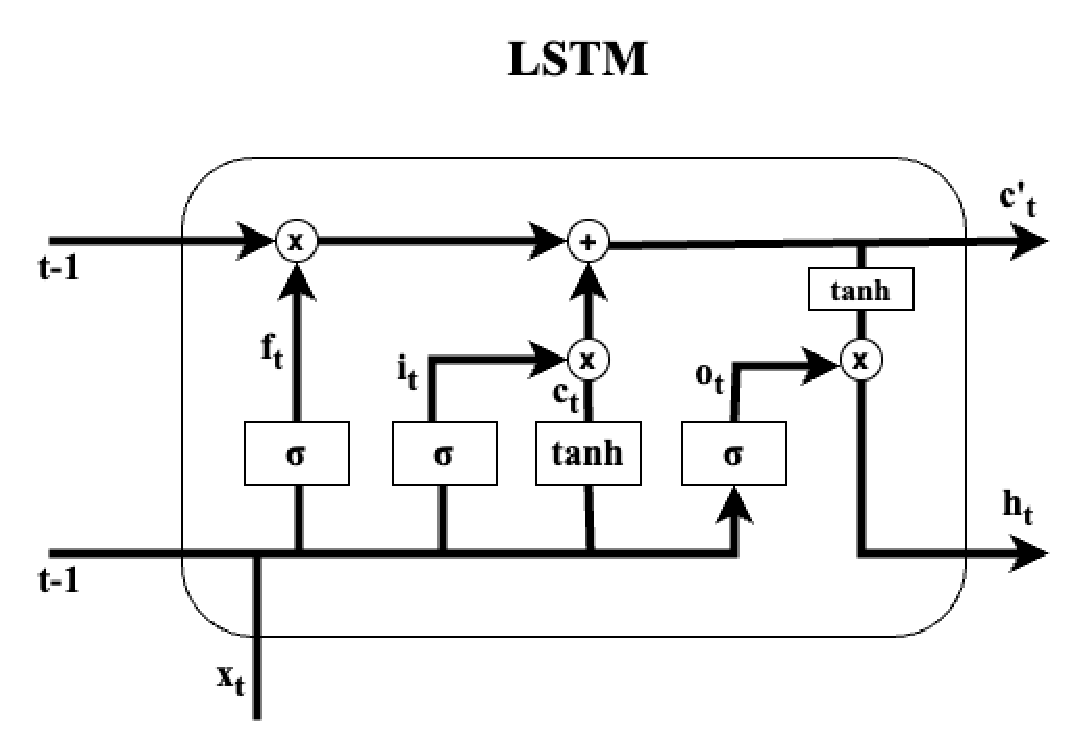
\includegraphics[width=0.8\linewidth]{LSTM.eps}
  \caption{Topology of a LSTM cell~\textcolor{red}{Is the pic taken from anywhere?}.}
  \label{fig:lstm}
\end{figure}

\section{System Model}

\textcolor{red}{final model used (some info)}
*
This model architecture comprises an LSTM layer, succeeded by two dense layers. It is specifically crafted for predicting time series data, where the input is structured with a shape of (10, 1). The model is trained using mean squared error as the loss function, Adam optimization algorithm, and employs Root Mean Squared Error as the evaluation metric. The LSTM layer is configured with 64 units, providing the model with the ability to capture sequential dependencies in the input data.

Additionally, the dense layers contribute to the model's expressiveness. The first dense layer possesses 8 units and utilizes the rectified linear unit (ReLU) activation function, introducing non-linearity to the model. The final layer is an output layer with a single unit and 'linear' activation, a suitable configuration for regression tasks. In terms of training parameters, the model uses a learning rate of 0.001, facilitating the convergence of the optimization process.
*

\textcolor{red}{algorithm as a figure}

\textcolor{red}{algorithm explanation}

\section{Results and Discussion}

\subsection{Evaluation Indices}

In this paper, Mean Squared Error (MSE) is used as an evaluation index to evaluate the prediction level of the model. This index is calculated as in (1) where $n$ is the number of data points, $y_i$ is the actual value, and $\hat{y}_i$ is the predicted value. In particular, the function \textit{(keras.losses.MeanSquaredError)} in Keras used for MSE calculation returns the average of the per-sample losses in a batch.

\begin{equation}
\text{MSE} = \frac{1}{n} \sum_{i=1}^{n} (y_i - \hat{y}_i)^2
\end{equation}

\subsection{Selecting Best Forecasting Methodology}

\textcolor{red}{use cleveref package to use \textbackslash cref\{\} for citing fig, table, section, etc.} Fig. x represents the traffic load of network data and network traffic for 15 years (Normal hours). The data consists of power in MW, consumed by each network for every hour in telecommunication.
*how we selected the best model type*

represents traffic load of network data and network traffic for 15 years (peak hours). The graph between the network data and network traffic in peak hours as well as in the normal hours has been shown with test data and training data. The normalization of network traffic can be achieved with the concept of XGBoost and prophet algor
*have attached the graph for all the three initial model types on COMED. if this is okay with you, will share the graphs for the Microsoft Dataset and the Temp Dataset as well*

\begin{table*}[ht]
  \caption{Performance of Different LSTM Models on Various Synthetic Datasets}
  \centering
  \resizebox{\textwidth}{!}{%
    \begin{tabular}{|*{9}{>{\centering\arraybackslash}p{0.11\textwidth}|}}
      \hline
      \textbf{Dataset/Model} & \textbf{Model 1} & \textbf{Model 2} & \textbf{Model 3} & \textbf{Model 4} & \textbf{Model 5} & \textbf{Model 6} & \textbf{Model 7} & \textbf{Model 8} \\
      \hline
      \textbf{Model 1} & 0.044 & 0.0054 & 0.2507 & 2.0302 & 0.6256 & 1.8354 & 1.186 & 1.1158 \\
      \hline
      \textbf{Model 2} & 0.3358 & 0.2262 & 0.2609 & 0.915 & 0.2613 & 0.855 & 0.486 & 0.4774 \\
      \hline
      \textbf{Model 3} & 0.5695 & 0.7270 & 0.4274 & 1.0624 & 0.3611 & 1.091 & 0.6027 & 0.593 \\
      \hline
      \textbf{Model 4} & 1.0267 & 0.5424 & 0.7875 & 0.5457 & 0.7711 & 1.3335 & 0.6144 & 0.9841 \\
      \hline
      \textbf{Model 5} & 0.5713 & 0.6027 & 0.4731 & 1.069 & 0.2857 & 1.011 & 0.5556 & 0.5418 \\
      \hline
      \textbf{Model 6} & 1.3595 & 1.1141 & 1.3407 & 1.2204 & 0.9841 & 1.2831 & 1.0261 & 1.0280 \\
      \hline
      \textbf{Model 7} & 0.5459 & 0.3503 & 0.2500 & 0.9837 & 0.2005 & 0.9108 & 0.4610 & 0.4590 \\
      \hline
      \textbf{Model 8} & 0.5806 & 0.2504 & 0.1865 & 0.9605 & 0.1640 & 0.8965 & 0.417 & 0.4134 \\
      \hline
    \end{tabular}%
  }
\end{table*}

\subsection{Model Performance Selection and Verification}
*finding best type of lstm model*

\begin{table*}[ht]
  \caption{Performance of Different Models on Various Synthetic Datasets}
  \centering
  \resizebox{\textwidth}{!}{%
    \begin{tabular}{|*{3}{>{\centering\arraybackslash}p{0.33\textwidth}|}}
      \hline
      \textbf{Dataset Type} & \textbf{Prophet Performance} & \textbf{LSTM Performance} \\
      \hline
      No Trend, No Seasonality & Does not trend correctly, trends in the opposite direction & Follows trend but does not account for the noise well \\
      \hline
      Upwards Trend, No Seasonality & Steadily trends upwards but not according to the data (underfits) & Follows trend but predicts widely off values when accounting for noise \\
      \hline
      Downwards Trend, No Seasonality & Trends appropriately but underfits, does not recognize dataset intricacies & Recognizes trend and seasonality but produces very inaccurate values due to noise \\
      \hline
      Upwards Trend, With Seasonality & Recognizes trend but not seasonality & Recognizes trend and seasonality well, performs satisfactorily with test data \\
      \hline
      Downwards Trend, With Seasonality & Recognizes trend but not seasonality & Recognizes trend and seasonality but produces very inaccurate values due to noise \\
      \hline
    \end{tabular}%
  }
\end{table*}
*add arima portion also here*

*will add graphs for all the lstm models on the real simulated data, need yogesh to share the data before that*

\section{Conclusions}
*
We investigated the effectiveness of a variety of deep learning approaches in predicting data traffic in cellular network nodes. In this paper, a scalable and easy-to-implement system that allows us to predict cell usage with greater accuracy is proposed. Among the explored methodologies, ARIMA was found to be a smaller network with fewer number of parameters but with a far too long time for training. Between Prophet and LSTM, the proposed LSTM model has less complexity and shows a smaller error difference. These two algorithms jointly resolves the issue of twining of the time series data provides the data modelling to support with network infrastructure. which can save enormous amount of energy. The system utilises machine learning techniques to improve traffic forecast and using the LSTM based system, we were able to limit the prediction MSE to xxx\%.

The final selected model presented xxx\% of accuracy for short-term prediction with the simulator data, which indicates that our system can, with a relatively small sample of data, rapidly and accurately forecast the network traffic passing through a node in a cellular network. This leads to major improvements in the operations of the network’s owner with a fairly low compute time required. As future work, the prediction of network traffic can be implemented using online models instead of the offline methodologies presented in this paper, updating the patterns of the traffic flow as data passes through the model. Another approach could be to use other forecasting methods such as those that consider more than one seasonality.

%The significance of this work is that predicting telecommunication traffic accurately can facilitate resource allocation in 5G networks. Future work will explore the effectiveness of the proposed models in predicting spatial dependencies along with temporal features by examining other datasets.
*

\begin{comment}
    
\begin{thebibliography}{1}
\bibitem{b1} Muhammad Faisal Iqbal et al., "Efficient prediction of network traffic for real-time applications", Journal of Computer Networks and Communications 2019, 2019.
\bibitem{b2} F. Toqué, M. Khouadjia, E. Come, M. Trepanier and L. Oukhellou, "Short & long term forecasting of multimodal transport passenger flows with machine learning methods," 2017 IEEE 20th International Conference on Intelligent Transportation Systems (ITSC), Yokohama, Japan, 2017, pp. 560-566, doi: 10.1109/ITSC.2017.8317939. keywords: {Forecasting;Predictive models;Conferences;Rail transportation;Smart cards;Computational modeling},
\bibitem{b3} N. Ramakrishnan and T. Soni, "Network Traffic Prediction Using Recurrent Neural Networks," 2018 17th IEEE International Conference on Machine Learning and Applications (ICMLA), Orlando, FL, USA, 2018, pp. 187-193, doi: 10.1109/ICMLA.2018.00035.
\bibitem{b4} Taylor SJ, Letham B. 2017. Forecasting at scale. PeerJ Preprints 5:e3190v2 https://doi.org/10.7287/peerj.preprints.3190v2
\bibitem{b5} D. Lee, D. Lee, M. Choi and J. Lee, "Prediction of Network Throughput using ARIMA," 2020 International Conference on Artificial Intelligence in Information and Communication (ICAIIC), Fukuoka, Japan, 2020, pp. 1-5, doi: 10.1109/ICAIIC48513.2020.9065083.
\bibitem{b6} S. McDonald, S. Coleman, T. M. McGinnity and Y. Li, "A hybrid forecasting approach using ARIMA models and self-organising fuzzy neural networks for capital markets," The 2013 International Joint Conference on Neural Networks (IJCNN), Dallas, TX, USA, 2013, pp. 1-7, doi: 10.1109/IJCNN.2013.6706965.
\bibitem{b7} M. Alizadeh, M. T. H. Beheshti, A. Ramezani and H. Saadatinezhad, "Network Traffic Forecasting Based on Fixed Telecommunication Data Using Deep Learning," 2020 6th Iranian Conference on Signal Processing and Intelligent Systems (ICSPIS), Mashhad, Iran, 2020, pp. 1-7, doi: 10.1109/ICSPIS51611.2020.9349573.
\bibitem{b8} R. Vinayakumar, K. P. Soman and P. Poornachandran, "Applying deep learning approaches for network traffic prediction," 2017 International Conference on Advances in Computing, Communications and Informatics (ICACCI), Udupi, India, 2017, pp. 2353-2358, doi: 10.1109/ICACCI.2017.8126198.
\bibitem{b9} I. Yenidoğan, A. Çayir, O. Kozan, T. Dağ and Ç. Arslan, "Bitcoin Forecasting Using ARIMA and PROPHET," 2018 3rd International Conference on Computer Science and Engineering (UBMK), Sarajevo, Bosnia and Herzegovina, 2018, pp. 621-624, doi: 10.1109/UBMK.2018.8566476.
\bibitem{b10} Paul Tune et al., "Internet traffic matrices: A primer", Recent Advances in Networking, vol. 1, pp. 1-56, 2013.
\bibitem{b11} C. Zhao, "Traffic Flow Prediction Model Based on Temporal Convolutional Network," 2023 17th International Conference on the Experience of Designing and Application of CAD Systems (CADSM), Jaroslaw, Poland, 2023, pp. 1-4, doi: 10.1109/CADSM58174.2023.10076492.
\bibitem{b12} J. Liu, H. Qu, M. Chen and Y. Gong, "Traffic Flow Prediction Based on Spatio-temporal Attention Block," 2022 International Conference on Machine Learning, Cloud Computing and Intelligent Mining (MLCCIM), Xiamen, China, 2022, pp. 32-39, doi: 10.1109/MLCCIM55934.2022.00014.
\bibitem{b13} D. Clemente, G. Soares, D. Fernandes, R. Cortesao, P. Sebastiao and L. S. Ferreira, "Traffic Forecast in Mobile Networks: Classification System Using Machine Learning," 2019 IEEE 90th Vehicular Technology Conference (VTC2019-Fall), Honolulu, HI, USA, 2019, pp. 1-5, doi: 10.1109/VTCFall.2019.8891348.
\bibitem{b14} D. Yuan and M. Zhang, "Citywide cellular traffic prediction based on densely connected convolutional neural networks", IEEE Communications Letters, vol. 22, no. 8, pp. 1656-1659, 2018.
\bibitem{b15} Guoqiang Yu and Zhang Changshui, "Switching ARIMA model based forecasting for traffic flow", 2004 IEEE International Conference on Acoustics Speech and Signal Processing, vol. 2, 2004.
\bibitem{b16} J. Lin, Y. Chen, H. Zheng, M. Ding, P. Cheng and L. Hanzo, "A data-driven base station sleeping strategy based on traffic prediction", IEEE Transactions on Network Science and Engineering, 2021.
\bibitem{b17} Y. Gao, M. Zhang, J. Chen, J. Han, D. Li and R. Qiu, "Accurate load prediction algorithms assisted with machine learning for network traffic", 2021 International Wireless Communications and Mobile Computing (IWCMC). IEEE, pp. 1683-1688, 2021.
\bibitem{b18} H. Tian, X. Zhou and J. Liu, "A Hybrid Network Traffic Prediction Model Based on Optimized Neural Network," 2017 18th International Conference on Parallel and Distributed Computing, Applications and Technologies (PDCAT), Taipei, Taiwan, 2017, pp. 284-287, doi: 10.1109/PDCAT.2017.00053.

\bibitem{b10} Xiaoguo Wang and Yuejing Liu, "ARIMA time series application to employment forecasting," 2009 4th International Conference on Computer Science and Education, Nanning, China, 2009, pp. 1124-1127, doi: 10.1109/ICCSE.2009.5228480.
\bibitem{b11} S. Bora and A. Hazarika, "Rainfall time series forecasting using ARIMA model," 2023 International Conference on Artificial Intelligence and Applications (ICAIA) Alliance Technology Conference (ATCON-1), Bangalore, India, 2023, pp. 1-5, doi: 10.1109/ICAIA57370.2023.10169493.
\bibitem{b12} S. Mehrmolaei and M. R. Keyvanpour, "Time series forecasting using improved ARIMA," 2016 Artificial Intelligence and Robotics (IRANOPEN), Qazvin, Iran, 2016, pp. 92-97, doi: 10.1109/RIOS.2016.7529496.
\bibitem{b13} Menculini, L.; Marini, A.; Proietti, M.; Garinei, A.; Bozza, A.; Moretti, C.; Marconi, M. Comparing Prophet and Deep Learning to ARIMA in Forecasting Wholesale Food Prices. Forecasting 2021, 3, 644-662. https://doi.org/10.3390/forecast3030040
\bibitem{b14} S. Sivaramakrishnan; Terrance Frederick Fernandez; R. G. Babukarthik; S. Premalatha, "4 Forecasting Time Series Data Using ARIMA and Facebook Prophet Models," in Big Data Management in Sensing: Applications in AI and IoT , River Publishers, 2021, pp.47-60.
\bibitem{b15} X. Pei, "Prophet algorithm-based power load forecasting model," 2023 IEEE 3rd International Conference on Electronic Technology, Communication and Information (ICETCI), Changchun, China, 2023, pp. 1498-1503, doi: 10.1109/ICETCI57876.2023.10176778.
\bibitem{b16} A. V. Nair and J. Narayanan, "Indian Stock Market Forecasting using Prophet Model," 2022 International Conference on Connected Systems and Intelligence (CSI), Trivandrum, India, 2022, pp. 1-7, doi: 10.1109/CSI54720.2022.9924117.


\end{thebibliography}
\end{comment}

\vspace{12pt}

\end{document}
